% Revised manuscript (v3). Historical baseline: paper/v2.2/main_v2.2.tex (unchanged).
% Evidence: Stage A (feature ablation) at commit dde1848; Stages B-D at 83585da; results archived in 630baad.
% Manuscript tables/figures: src/analysis/report_pub.py (see paper/revision_v3/generated/manifest.json).
% Tables are generated (generated/*.tex); do not edit numbers in them by hand.
\documentclass[a4paper,fleqn]{cas-sc}
\usepackage{booktabs}
\usepackage{placeins}
\usepackage{amsmath}
\usepackage{xcolor}
\usepackage[authoryear]{natbib}
\usepackage{hyperref}
\hypersetup{colorlinks=true,linkcolor=blue,citecolor=blue,urlcolor=cyan}
\usepackage{lastpage}
% cas-common writes the page total at \AtEndDocument, before deferred floats are output; use LastPage instead.
\AtBeginDocument{\def\lastpage{\pageref*{LastPage}}}
\usepackage[pagewise]{lineno}
\linenumbers
\shorttitle{UQ for ship motion forecasting under an operating-condition shift}
\shortauthors{Asan et al.}
\begin{document}
\let\WriteBookmarks\relax

\title [mode = title]{A controlled benchmark of uncertainty quantification for multi-step ship motion forecasting under an operating-condition shift}

\author[1]{Vedat Mert Asan}[orcid=0009-0003-7134-9728]
\cormark[1]
\ead{mert.asan@taltech.ee}
\author[1]{Mihkel K\~{o}rgesaar}
\author[1]{Kristjan Tabri}
\cortext[cor1]{Corresponding author}
\affiliation[1]{organization={TalTech, Kuressaare College, Naval Architecture and Hydrodynamics Research Group},
city={Kuressaare},
country={Estonia}}

\begin{abstract}
Learned forecasters of ship motion are usually evaluated by point accuracy on data resembling their training data. We report a controlled benchmark of how uncertainty estimates for 30-step (30~s) forecasts of five motion states behave in distribution and under an operating-condition shift, using the simulated patrol-vessel dataset of Baier and Staab. Windows are built within one-hour recordings; models are trained on 48 recordings, calibrated on 9 further training recordings excluded from fitting, selected on 9 validation recordings and tested on 30 in-distribution (ID) recordings and on 29 separately provided recordings at higher speeds and propeller shaft speeds (out-of-distribution, OOD). The OOD results are exploratory, because these recordings informed model selection in an earlier version of this study. Seven point forecasters, including closed-form ridge regression and a last-value baseline, and four uncertainty representations (absolute residuals, 5-member deep-ensemble spread, 200-pass Monte Carlo dropout spread and a Gaussian likelihood head) are compared with three training repeats, split-conformal calibration and recording-level bootstrap intervals. In distribution, ridge regression and the neural forecasters have similar observed channel-averaged normalised errors (0.31--0.34), all lower than last-value persistence (0.49); every split-conformal construction covers about 93\% of observations at a nominal 90\%, whereas uncalibrated ensemble and dropout bands cover 26--71\%. Under the shift, normalised errors rise to 0.93--1.01 for all learned models. Split-conformal intervals with an absolute-residual score cover 50--53\%, while scores normalised by ensemble or dropout spread cover 70--78\% with wider intervals and lower interval scores; normalisation by the Gaussian standard deviation brings no gain. In post hoc, descriptive matched comparisons, the coverage gain of the ensemble- and dropout-normalised scores persisted when the point predictor was held fixed. No construction reaches nominal coverage under the shift.
\end{abstract}

\begin{highlights}
\item Recording-aware benchmark of uncertainty for 30-s ship motion forecasts
\item Ridge regression and neural forecasters show similar in-distribution errors
\item All split-conformal variants over-cover in distribution at a 90\% target
\item Ensemble- or dropout-normalised conformal scores cover 70--78\% under the shift
\item No construction reaches nominal coverage under the exploratory OOD shift
\end{highlights}

\begin{keywords}
Ship motion prediction \sep Uncertainty quantification \sep Conformal prediction \sep Deep ensembles \sep Distribution shift \sep Benchmark
\end{keywords}

\maketitle

% ============================================================
\section{Introduction}
\label{sec:intro}

Multi-step forecasting of ship motion---the prediction of a sequence of future vessel states over a finite horizon---supports trajectory planning, motion control and decision-making in marine operations \citep{fossen2011handbook}. High-fidelity hydrodynamic simulation can produce such forecasts, but its computational cost is generally incompatible with onboard real-time use \citep{thombre2022autonomous}, which has motivated learned, data-driven predictors. A learned predictor's accuracy is demonstrated only for the conditions represented in its training data, whereas vessels operate over a range of speeds, loading conditions and sea states. A forecast that is accompanied by a statement of its uncertainty is therefore only useful if that statement remains informative when conditions change.

Neural network predictors for ship motion include data-driven system identification of six-degree-of-freedom motion in waves \citep{silva2022ship}, data-driven vessel-motion models augmented with physics-based information \citep{schirmann2022datadriven} and comparisons of physics-informed data-driven architectures \citep{schirmann2023comparison}, recurrent models combined with Gaussian-process regression for short-term attitude prediction \citep{sun2022shipmotion}, data-driven multi-step roll prediction in high sea states \citep{zhang2023roll}, optimised LSTM models using principal components of wave height \citep{gong2025wavelet}, hybrid physics and deep-learning models for vehicle-state prediction \citep{baier2021hybrid}, and deep learning for six-degree-of-freedom motion in real sea conditions \citep{zhang2023deep}. These studies, as summarised here, are evaluated primarily through point-forecast accuracy.

Probabilistic ship-motion forecasting has begun to appear. \citet{kim2025mcdropoutroll} applied Monte Carlo (MC) dropout to LSTM and Transformer roll-motion predictors trained on hydrodynamic simulations and validated on ferry voyage data, and evaluated interval coverage and width. Outside the marine domain, \citet{ovadia2019can} showed on image, text and tabular tasks that uncertainty estimates that appear calibrated in distribution can degrade substantially under dataset shift, and that the ranking of methods need not be stable across shift severity. Conformal prediction provides distribution-free marginal coverage when calibration and test data are exchangeable \citep{vovk2005algorithmic, angelopoulos2023conformal}; it has been extended to multi-horizon time-series forecasting \citep{stankeviciute2021conformal}, to scores normalised by an estimate of local difficulty \citep{lei2018distribution}, to covariate shift by re-weighting \citep{tibshirani2019conformal} and to online adaptation under distribution shift \citep{gibbs2021adaptive}. Deep ensembles \citep{lakshminarayanan2017}, MC dropout \citep{gal2016dropout} and likelihood models with post hoc calibration \citep{kuleshov2018calibrated} are widely used alternatives for representing predictive uncertainty.

What is missing for multi-step, multivariate ship motion is a controlled comparison of these practical constructions on a common task, with a common calibration set, common nominal levels and scores that account for both coverage and interval width, evaluated both in distribution and under an explicitly characterised change of operating conditions. This paper provides such a comparison. It does not propose a new algorithm. Its contributions are:
\begin{enumerate}
    \item A reproducible benchmark protocol for the simulated patrol-vessel dataset of \citet{baier2022darus}: recording-aware windowing, a calibration split excluded from fitting, training-only standardisation, a predeclared feature decision, three training repeats, and recording-level bootstrap intervals, with published split manifests, seeds and checkpoint provenance.
    \item A comparison of seven point forecasters, including closed-form ridge regression and last-value persistence, in distribution and under the shift, using channel-wise errors in physical units and a channel-averaged normalised error.
    \item A comparison of four uncertainty representations---absolute residuals, deep-ensemble spread, MC-dropout spread and a Gaussian likelihood head---both uncalibrated and calibrated by split conformal prediction on the same calibration recordings, with coverage reported together with width and interval score at four predeclared nominal levels, and with predeclared paired comparisons that separate backbone effects from differences between constructions.
\end{enumerate}

Section~\ref{sec:methods} describes the data, task, models, uncertainty constructions and evaluation protocol; Section~\ref{sec:results} reports results; Section~\ref{sec:discussion} discusses their interpretation and limitations; Section~\ref{sec:conclusions} concludes.

% ============================================================
\section{Materials and methods}
\label{sec:methods}

\subsection{Dataset and operating-condition shift}
\label{sec:dataset}

We use the publicly available DaRUS deposit of \citet{baier2022darus}, which contains 125 one-hour \emph{simulations} of a patrol ship with extended rudder propellers performing random manoeuvres in four degrees of freedom (surge, sway, yaw, roll), with wind forces following Isherwood's model and wave-induced motion generated from a JONSWAP spectrum, as described in the deposit metadata; according to \citet{baier2021hybrid}, the simulator extends the four-degree-of-freedom patrol-ship model of Perez, Ross and Fossen from the Marine Systems Simulator toolbox. The deposit provides 96 routine recordings, partitioned by the providers into 57 training, 9 validation and 30 test recordings, and 29 separately provided out-of-distribution (OOD) recordings. Each recording contains 3601 samples at a verified sampling interval of 1~s, without gaps, repeated samples or missing values. The files contain twelve columns: elapsed time $t$ (s); propeller shaft speed $n$ (stated as 1/s in the dataset documentation\footnote{The deposit README lists $n$ in 1/s. The recorded values (226--1612 in the training recordings and up to 2233 in the OOD recordings) are implausibly large for revolutions per second of a patrol-vessel propeller and would be consistent with revolutions per minute, but we found no primary source that establishes the convention. We therefore report the values as provided; $n$ enters the models only after standardisation, so no result depends on its unit.}); left and right azimuth angles $\delta_l,\delta_r$ (rad); wind speed $V_w$ (m/s) and the cosine and sine of the relative wind angle; surge and sway velocities $u,v$ (m/s); roll and yaw rates $p,r$ (rad/s); and roll angle $\phi$ (rad). No wave elevation, wave force or sea-state parameters are included.

The OOD recordings differ from the training recordings in operating condition: surge velocity spans 3.45--13.44~m/s (mean 8.50~m/s) against 0.95--9.25~m/s (mean 5.64~m/s), and propeller shaft speed (in the dataset's stated unit) has mean 1582 and maximum 2233 against 1040 and 1612 in the training recordings (ratios 1.52 and 1.39), so the OOD inputs extrapolate beyond the training range of a control input. Wind speed has similar means (1.81 vs.\ 1.97~m/s). Because sea-state parameters are not available in the files, we refer to the shift as a \emph{combined operating-condition shift} rather than a sea-state shift.

\subsection{Forecasting task and windows}
\label{sec:task}

Given a history of $H=30$ samples (30~s) of $F=11$ input channels, a model predicts the next $T=30$ samples of the $D=5$ target states $[u,v,p,r,\phi]$. Windows are constructed with stride 1 \emph{within} each recording, never across recording boundaries, giving $3601-60+1=3542$ windows per recording. The five targets are also inputs (their past values); no future input values are used.

\subsection{Data roles, preprocessing and feature set}
\label{sec:splits}

Table~\ref{tab:roles} lists the data roles. Nine of the 57 deposit training recordings were reserved for calibration only, selected by a fixed-seed random draw (NumPy \texttt{default\_rng(20261001)}) before any model of the present benchmark was trained; the remaining 48 recordings are used for fitting. The deposit validation recordings are used for checkpoint selection, early stopping, the ridge penalty and the feature decision. In the present benchmark, the ID and OOD test recordings are used only for reporting; the OOD recordings had, however, been consulted for model selection in an earlier version of this study (Section~\ref{sec:limitations}). A predeclared representativeness check comparing per-recording means and standard deviations of all inputs and targets between calibration and fitting recordings did not meet its $|\text{SMD}|\le 0.5$ criterion (maximum 0.84, $\delta_l$ standard deviation); the calibration recordings are somewhat slower on average (standardised mean difference $-0.52$ in mean $u$). The draw was nevertheless retained, as decided before evaluation, and the imbalance is reported rather than corrected.

% generated by src.analysis.report_pub from experiments/manifests; do not edit by hand
\begin{table}[tbp]
\centering\footnotesize
\caption{Data roles. Windows: history 30~s, horizon 30~s, stride 1, within recordings (3{,}542 per recording).}
\label{tab:roles}
\begin{tabular}{lrrl}
\toprule
Role & Recordings & Windows & Use \\
\midrule
Fit & 48 & 170{,}016 & gradient updates; scaler fitting \\
Calibration & 9 & 31{,}878 & conformal thresholds; spread floor \\
Validation & 9 & 31{,}878 & checkpoint selection, early stopping, feature decision, ridge penalty \\
ID test & 30 & 106{,}260 & reporting \\
OOD test & 29 & 102{,}718 & reporting (exploratory; consulted in an earlier version) \\
\bottomrule
\end{tabular}
\end{table}


Inputs and targets are standardised per channel with means and standard deviations computed on the fitting recordings only; losses are computed on standardised targets, so the five targets carry equal weight, and all reported errors and interval widths are transformed back to physical units. The elapsed-time column restarts at zero in every recording and encodes position within a recording rather than a physical state. A predeclared validation-only rule decided whether to keep it: it would be kept only if it reduced the best validation loss by more than 2\% for both an LSTM and an MLP. It increased the validation loss slightly for both (by 0.19\% and 0.35\%), so all models use the eleven remaining inputs.

\subsection{Point forecasters}
\label{sec:backbones}

All neural models map the input window to the full $30\times5$ output in one forward pass (non-autoregressive):
\begin{itemize}
\item \textbf{LSTM seq2seq} \citep{hochreiter1997lstm, sutskever2014seq2seq}: two-layer LSTM encoder (128 units); a two-layer LSTM decoder initialised with the encoder state and fed zero inputs for 30 steps (no feedback of predictions); a linear projection to the five targets.
\item \textbf{GRU seq2seq} \citep{cho2014gru}: the same structure with GRU cells.
\item \textbf{TCN} \citep{bai2018tcn}: three residual blocks of dilated causal convolutions (64 channels, kernel 3, dilations 1, 2, 4, dropout 0.1) followed by a linear map from the flattened feature sequence to the output.
\item \textbf{MLP}: three fully connected layers (330 $\to$ 256 $\to$ 256 $\to$ 150) with ReLU activations.
\item \textbf{Linear (SGD)}: a single linear map from the flattened window (330 values) to the 150 outputs, trained like the networks.
\item \textbf{Ridge}: the same linear map fitted in closed form; the penalty was chosen on the validation recordings from a predeclared grid, which selected the unpenalised solution (the edge of the grid).
\item \textbf{Naive}: repetition of the last observed target values.
\end{itemize}
Parameter counts are given in Table~\ref{tab:baselines}.

\subsection{Training}
\label{sec:training}

Models were trained with Adam \citep{kingma2015adam} (learning rate $10^{-3}$, batch 256, no weight decay) on the mean squared error of standardised targets, or on the Gaussian negative log-likelihood (including the $\tfrac12\log 2\pi$ constant) for the likelihood models. Training ran for at most 100 epochs with early stopping (patience 10) on the validation objective, and the checkpoint with the lowest validation loss was retained. Every run used a recorded seed. Each trained configuration was run in three independent repeats; an ensemble repeat consists of five freshly initialised members with distinct seeds, and member 0 of each repeat serves as that repeat's single-model forecaster. Ridge regression and persistence are deterministic and were fitted once; for them, recording-level intervals are reported but no between-seed variation exists. Every trained run ended by early stopping: the best validation epoch was 2--5 for the recurrent models, the TCN and the Gaussian LSTM, 3--10 for the MLP and the Gaussian MLP, 16--32 for the MLP with dropout and 22--49 for the linear model trained by SGD. We report the validation-selected checkpoints; early stopping does not establish that optimisation has converged, and the reasons for the early validation optimum were not investigated.

\subsection{Uncertainty representations and calibration}
\label{sec:uq-methods}

For a window, let $\mu$ denote the point forecast and $s$ a non-negative spread, both of shape $30\times5$. We consider four representations:
\begin{itemize}
\item \textbf{Absolute residual}: $\mu$ from a single point forecaster; no spread.
\item \textbf{Deep ensemble} \citep{lakshminarayanan2017}: $\mu$ is the mean of five members and $s$ their sample standard deviation (denominator $N-1$).
\item \textbf{MC dropout} \citep{gal2016dropout}: models trained with dropout probability 0.2; at inference, dropout remains active and $\mu$ and $s$ are the mean and sample standard deviation over 200 stochastic passes. In the LSTM, dropout acts only between the two stacked layers of the encoder and decoder; in the MLP, after each hidden layer.
\item \textbf{Gaussian likelihood}: an LSTM or MLP head that outputs $\mu$ and $\log\sigma^2$ (clamped to $[-10,5]$), with $s=\sigma$.
\end{itemize}

\paragraph{Uncalibrated bands.} For the three representations with a spread, we report $\mu \pm z_{1-\alpha/2}\, s$, where $z$ is a standard normal quantile. This is a Gaussian-reference band; its nominal level is not a coverage guarantee.

\paragraph{Split conformal prediction.} All calibrated intervals use split conformal prediction \citep{vovk2005algorithmic, angelopoulos2023conformal} on the nine calibration recordings ($n=31{,}878$ windows) with one of two scores:
\begin{align*}
\text{absolute residual (AR-SCP):}\quad & S = |y-\mu|, & [L,U] &= \mu \pm q,\\
\text{spread-normalised:}\quad & S = |y-\mu|/\max(s, f), & [L,U] &= \mu \pm q\,\max(s,f),
\end{align*}
where the spread-normalised score \citep{lei2018distribution} is used with the ensemble spread (EN-SCP), the MC-dropout spread (DN-SCP) or the Gaussian $\sigma$ (GN-SCP). The threshold $q$ is the $k$-th smallest calibration score with $k=\lceil (n+1)(1-\alpha)\rceil$, computed separately for every forecast step and channel (150 thresholds; primary construction). A per-channel variant pooling the horizon is stored as a secondary result. The floor is $f_d = 10^{-3}\max(\bar s_d, \mathrm{sd}(y_d))$ per channel $d$, where $\bar s_d$ is the mean spread and $\mathrm{sd}(y_d)$ the standard deviation of the targets, both computed on the calibration recordings; the calibration recordings therefore determine both the thresholds and the floor. The floor was fixed before evaluation, and its sensitivity is reported in Section~\ref{sec:results-id}.

Under exchangeability of calibration and test windows, this construction guarantees marginal coverage of at least $1-\alpha$ for a new scalar prediction. In this study the windows overlap heavily and come from nine calibration recordings, so exchangeability with the test windows is not established even in distribution, and it is violated by design under the shift. We therefore report \emph{nominal} levels, \emph{empirical} coverage and the formal \emph{guarantee} as distinct quantities and do not claim the guarantee for these data. All intervals are marginal: they target the coverage of individual scalar predictions (one step, one channel), not simultaneous coverage of a whole trajectory.

\subsection{Metrics and statistical analysis}
\label{sec:eval-protocol}

Point accuracy is reported as the RMSE of each channel in physical units and as a channel-averaged normalised RMSE (the mean over channels of the RMSE divided by the standard deviation of that channel's targets in the fitting recordings, the same scale used for standardisation). A pooled RMSE over channels with different units is not used to rank models. For intervals we report the empirical marginal coverage over all windows, steps and channels, the mean interval width divided per channel by the training-target standard deviation and averaged over channels, and the interval (Winkler) score \citep{gneiting2007scoring}
\[
\mathrm{IS}_\alpha(L,U;y) = (U-L) + \tfrac{2}{\alpha}(L-y)\,\mathbb{1}\{y<L\} + \tfrac{2}{\alpha}(y-U)\,\mathbb{1}\{y>U\},
\]
normalised in the same way (lower is better). The nominal levels 0.5, 0.8, 0.9 (primary) and 0.95 were fixed in advance. We also report simultaneous whole-trajectory coverage as a descriptive quantity.

Because windows overlap, the resampling unit is the recording. For every method and split, 95\% intervals are percentile intervals from a cluster bootstrap that resamples whole test recordings (2000 draws); within each draw, the statistic is averaged over the three training repeats (or taken from the single fit for ridge and persistence). These intervals describe uncertainty due to the finite set of test recordings. Variation between training repeats is reported separately as a standard deviation. Sixteen paired comparisons were predeclared (each spread-based construction vs.\ AR-SCP on the same backbone, MLP vs.\ LSTM within each construction, and calibrated vs.\ uncalibrated for each spread); they use identical recordings and shared bootstrap draws. No multiplicity adjustment is applied, and paired intervals are interpreted descriptively. Analyses not in the predeclared specification are labelled \emph{post hoc}.

\subsection{Protocol, provenance and computation}
\label{sec:protocol}

The protocol of the present benchmark (data roles, preprocessing, training, constructions, levels, bootstrap specification, table and figure rules) was frozen before any of its models was evaluated on the ID or OOD test recordings; this does not undo the earlier use of the OOD recordings noted in Section~\ref{sec:limitations}. A timing pilot scored only the validation recordings. The benchmark was then run in gated stages with automated checks between stages (window and optimiser-step counts, calibration membership, scaler and split hashes, member provenance of every ensemble): the feature ablation at code version \texttt{dde1848}, and training, evaluation and analysis at \texttt{83585da}. The two versions have identical training, data, model and evaluation code; the later version adds the analysis scripts, a stricter repeat-count check in the bootstrap, run records, and a changed comment in the configuration files. Training and evaluation used NVIDIA L40 GPUs (1.55 GPU-hours for the benchmark, excluding a 0.08 GPU-hour timing pilot); analyses ran on a CPU. Every table and figure in Section~\ref{sec:results} is generated from stored outputs by scripts in the code repository.

% ============================================================
\section{Results}
\label{sec:results}

\subsection{Point accuracy}
\label{sec:results-point}

% generated by src.analysis.report_pub from frozen v3 outputs; do not edit by hand
\begin{table*}[tbp]
\centering
\footnotesize
\caption{Deterministic point accuracy (ID test: 30 recordings; OOD test: 29 recordings, exploratory). Normalised RMSE = mean over the five channels of RMSE divided by the training-target standard deviation of that channel (dimensionless). Values are means over training repeats; brackets give the 95\% percentile interval of a cluster bootstrap that resamples whole recordings (2000 draws) and averages over repeats, i.e.\ uncertainty due to the finite set of test recordings, not across-seed variation. Ridge and naive are single deterministic fits.}
\label{tab:baselines}
\begin{tabular}{lrrcc}
\toprule
Model & Parameters & Repeats & ID normalised RMSE [95\% CI] & OOD normalised RMSE [95\% CI] \\
\midrule
LSTM seq2seq & 406,149 & 3 & 0.325 [0.279, 0.373] & 0.947 [0.924, 0.971] \\
GRU seq2seq & 304,773 & 3 & 0.314 [0.268, 0.361] & 0.927 [0.904, 0.951] \\
TCN & 352,854 & 3 & 0.328 [0.282, 0.374] & 0.971 [0.947, 0.997] \\
MLP & 189,078 & 3 & 0.322 [0.277, 0.368] & 0.940 [0.917, 0.964] \\
Linear (SGD) & 49,650 & 3 & 0.336 [0.290, 0.384] & 1.006 [0.979, 1.033] \\
Linear (ridge, closed form) & 49,650 & 1 & 0.328 [0.281, 0.375] & 0.987 [0.960, 1.014] \\
Naive (last value) & 0 & 1 & 0.494 [0.419, 0.568] & 1.243 [1.211, 1.276] \\
\bottomrule
\end{tabular}
\end{table*}

% generated by src.analysis.report_pub from frozen v3 outputs; do not edit by hand
\begin{table*}[tbp]
\centering
\footnotesize
\caption{Per-channel RMSE in physical units ($u$: m\,s$^{-1}$, $v$: m\,s$^{-1}$, $p$: rad\,s$^{-1}$, $r$: rad\,s$^{-1}$, $\phi$: rad), mean over training repeats; recording-bootstrap intervals for every entry are in the accompanying CSV (\texttt{experiments/analysis/v3/bootstrap}). The channels differ by up to two orders of magnitude, so no pooled error is used for ranking.}
\label{tab:channel-rmse}
\begin{tabular}{lrrrrrrrrrr}
\toprule
& \multicolumn{5}{c}{ID test} & \multicolumn{5}{c}{OOD test (exploratory)} \\ \cmidrule(lr){2-6}\cmidrule(lr){7-11}
Model & $u$ & $v$ & $p$ & $r$ & $\phi$ & $u$ & $v$ & $p$ & $r$ & $\phi$ \\
\midrule
LSTM seq2seq & 0.1844 & 0.0579 & 0.0052 & 0.0047 & 0.0082 & 0.7158 & 0.3599 & 0.0074 & 0.0200 & 0.0256 \\
GRU seq2seq & 0.1471 & 0.0523 & 0.0052 & 0.0045 & 0.0078 & 0.6022 & 0.3580 & 0.0074 & 0.0202 & 0.0243 \\
TCN & 0.1695 & 0.0599 & 0.0052 & 0.0048 & 0.0082 & 0.6378 & 0.3681 & 0.0076 & 0.0206 & 0.0280 \\
MLP & 0.1670 & 0.0566 & 0.0052 & 0.0047 & 0.0080 & 0.5985 & 0.3655 & 0.0075 & 0.0203 & 0.0250 \\
Linear (SGD) & 0.1366 & 0.0658 & 0.0052 & 0.0049 & 0.0098 & 0.5501 & 0.3957 & 0.0077 & 0.0203 & 0.0347 \\
Linear (ridge, closed form) & 0.1179 & 0.0616 & 0.0052 & 0.0048 & 0.0096 & 0.5240 & 0.3860 & 0.0076 & 0.0201 & 0.0339 \\
Naive (last value) & 0.3191 & 0.0968 & 0.0083 & 0.0056 & 0.0131 & 0.7482 & 0.5109 & 0.0111 & 0.0228 & 0.0380 \\
\bottomrule
\end{tabular}
\end{table*}


In distribution, the neural forecasters and both linear models have similar observed channel-averaged normalised RMSE (0.314--0.336, Table~\ref{tab:baselines}) with overlapping recording-level intervals; last-value persistence has a higher error (0.494). The observed error of closed-form ridge regression (0.328) lies within the range of the neural models. Overlapping intervals do not establish equivalence, and the benchmark contains no predeclared paired comparison with ridge; it therefore provides no evidence either way on whether the neural models are more accurate than ridge. Per channel (Table~\ref{tab:channel-rmse}), ridge has the lowest ID surge error (0.118~m/s against 0.147--0.184~m/s for the networks), whereas the networks have lower sway and roll-angle errors.

Under the operating-condition shift, the normalised RMSE of every learned model roughly triples (0.927--1.006), and persistence degrades to 1.243. The MLP has a lower OOD normalised RMSE than the LSTM by $-0.007$ [$-0.009$, $-0.005$] (predeclared paired comparison), a small difference relative to the level of about 0.94. For the learned models, the largest OOD errors in physical units occur in surge (0.52--0.72~m/s) and sway (0.36--0.40~m/s).

\subsection{In-distribution interval quality}
\label{sec:results-id}

% generated by src.analysis.report_pub from frozen v3 outputs; do not edit by hand
\begin{table*}[tbp]
\centering
\footnotesize
\caption{Interval quality at nominal 90\% on the ID test (30 recordings). Coverage = marginal coverage of individual scalar predictions (all windows, 30 steps, 5 channels); width and interval score (Winkler score, $\alpha=0.1$) are divided per channel by the training-target standard deviation and averaged over channels (dimensionless; lower interval score is better). Brackets: 95\% recording-level cluster-bootstrap intervals; last column: standard deviation of coverage across the three training repeats (percentage points), a separate source of variation. AR-SCP rows use the member-0 model of each repeat (single models); EN-, DN- and GN-SCP use the ensemble mean, dropout mean and Gaussian mean with a score normalised by the corresponding spread.}
\label{tab:uq-id}
\begin{tabular}{llcccc}
\toprule
Construction & Backbone & Coverage \% [95\% CI] & Norm.\ width [95\% CI] & Norm.\ interval score [95\% CI] & Seed SD (pp) \\
\midrule
\multicolumn{6}{l}{\emph{Split conformal (calibrated on 9 held-out training recordings)}} \\
AR-SCP & LSTM & 92.8 [90.9, 94.4] & 1.01 [1.01, 1.01] & 1.59 [1.39, 1.84] & 0.1 \\
AR-SCP & GRU & 93.0 [91.1, 94.7] & 0.97 [0.97, 0.97] & 1.55 [1.35, 1.80] & 0.1 \\
AR-SCP & TCN & 92.8 [91.0, 94.4] & 1.01 [1.01, 1.01] & 1.60 [1.40, 1.84] & 0.1 \\
AR-SCP & MLP & 92.8 [91.0, 94.4] & 1.00 [1.00, 1.00] & 1.58 [1.38, 1.82] & 0.1 \\
AR-SCP & Linear (SGD) & 92.8 [91.1, 94.4] & 1.04 [1.04, 1.04] & 1.64 [1.43, 1.88] & 0.1 \\
AR-SCP & Ridge & 93.0 [91.3, 94.5] & 1.01 [1.01, 1.01] & 1.61 [1.40, 1.86] & -- \\
AR-SCP & Naive & 91.8 [90.1, 93.5] & 1.52 [1.52, 1.52] & 2.42 [2.09, 2.81] & -- \\
EN-SCP & LSTM & 93.4 [92.7, 94.2] & 1.20 [1.09, 1.33] & 1.63 [1.45, 1.83] & 0.1 \\
EN-SCP & MLP & 93.4 [92.6, 94.3] & 1.17 [1.10, 1.25] & 1.61 [1.46, 1.79] & 0.2 \\
DN-SCP & LSTM & 93.5 [92.3, 94.7] & 1.05 [1.00, 1.11] & 1.54 [1.37, 1.73] & 0.1 \\
DN-SCP & MLP & 93.2 [92.2, 94.1] & 1.03 [0.97, 1.10] & 1.49 [1.34, 1.67] & 0.0 \\
GN-SCP & LSTM & 92.7 [92.4, 93.1] & 0.93 [0.83, 1.05] & 1.35 [1.21, 1.52] & 0.1 \\
GN-SCP & MLP & 92.6 [92.3, 93.0] & 0.90 [0.80, 1.01] & 1.30 [1.17, 1.45] & 0.1 \\
\midrule
\multicolumn{6}{l}{\emph{Uncalibrated bands $\mu \pm z_{0.95}\,s$}} \\
Ensemble raw & LSTM & 59.6 [57.8, 61.4] & 0.22 [0.20, 0.23] & 2.36 [1.98, 2.79] & 1.4 \\
Ensemble raw & MLP & 61.0 [58.9, 63.2] & 0.22 [0.21, 0.24] & 2.30 [1.92, 2.74] & 1.3 \\
Dropout raw & LSTM & 25.7 [24.4, 27.1] & 0.08 [0.08, 0.08] & 3.16 [2.69, 3.69] & 1.6 \\
Dropout raw & MLP & 71.0 [69.3, 72.7] & 0.35 [0.34, 0.37] & 2.26 [1.89, 2.67] & 0.4 \\
Gaussian raw & LSTM & 93.7 [93.4, 93.9] & 1.00 [0.89, 1.12] & 1.36 [1.22, 1.53] & 0.6 \\
Gaussian raw & MLP & 93.2 [92.9, 93.5] & 0.94 [0.84, 1.05] & 1.31 [1.18, 1.46] & 0.6 \\
\bottomrule
\end{tabular}
\end{table*}


All split-conformal constructions with learned forecasters attain empirical ID coverage of 92.6--93.5\% at a nominal 90\% (91.8\% with persistence; Table~\ref{tab:uq-id}), and every recording-level interval excludes 90\%. This over-coverage appears at all nominal levels (61--65\% at 50\%, 86--87\% at 80\% and 96--97\% at 95\%; Fig.~\ref{fig:levels} and Table~\ref{tab:o1}), decreases with forecast step (Fig.~\ref{fig:horizon}) and is concentrated in surge (94--96\%) and, substantially, in sway (98.5--99\% at a nominal 90\%), whereas roll rate, yaw rate and roll angle are within about one percentage point of the nominal level (Table~\ref{tab:channel-coverage}). At 90\%, the coverage range across the three training repeats is at most 0.4 percentage points for the split-conformal constructions and 1.2 points for the uncalibrated Gaussian bands, smaller than the recording-level uncertainty. The calibration recordings are somewhat slower than the other recordings (Section~\ref{sec:splits}); whether this contributes to the over-coverage was not tested.

The uncalibrated ensemble bands cover 60--61\% and the uncalibrated dropout bands 26\% (LSTM) and 71\% (MLP) at a nominal 90\%, whereas the uncalibrated Gaussian bands already cover 93--94\%. In distribution, GN-SCP has the narrowest intervals among the split-conformal constructions (normalised width 0.93 and 0.90, against 0.98--1.04 for AR-SCP with the learned forecasters, 1.03--1.05 for DN-SCP and 1.17--1.20 for EN-SCP) together with the lowest interval scores (1.35 and 1.30, against 1.49--1.64), at similar coverage. The simultaneous coverage of complete 30-step, five-channel trajectories is much lower than the marginal coverage (0.16--0.40; Table~\ref{tab:o1}).

The spread floor was essentially inactive: across all spread-based evaluations, channels, levels and splits, at most $6.3\times10^{-6}$ of calibration spreads were floored. Replacing the factor $10^{-3}$ by $10^{-4}$ or $10^{-2}$ changed coverage by at most 0.25 percentage points and normalised width by at most 0.05.

\begin{figure}[tbp]
\centering
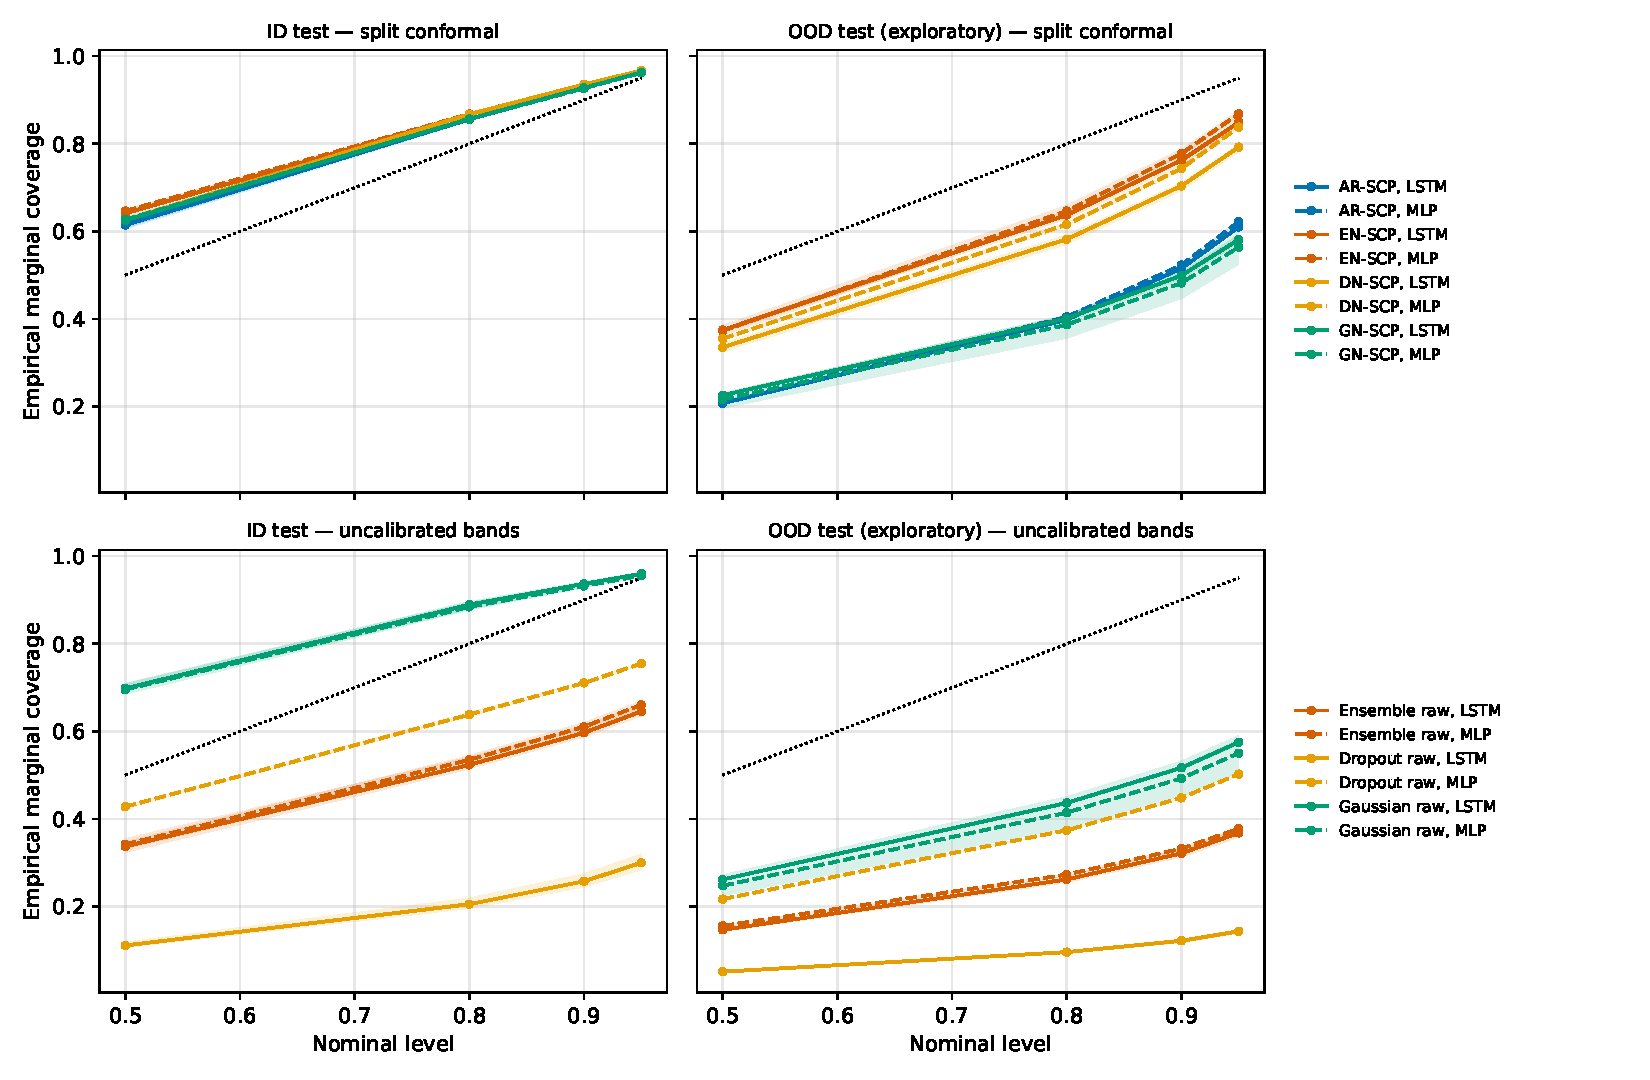
\includegraphics[width=0.92\linewidth]{generated/fig_coverage_levels.pdf}
\caption{Empirical marginal coverage against nominal level for split-conformal constructions (top) and uncalibrated bands (bottom), ID test (left) and OOD test (right, exploratory). Lines: mean over three training repeats; shaded bands: minimum--maximum over the three repeats (seed range, not a recording-level confidence interval). Dotted line: nominal level. Colour: construction; solid: LSTM; dashed: MLP.}
\label{fig:levels}
\end{figure}

% generated by src.analysis.report_pub from frozen v3 outputs; do not edit by hand
\begin{table*}[tbp]
\centering
\footnotesize
\caption{Per-channel marginal coverage (\%) at nominal 90\%, means over repeats. Recording-bootstrap intervals for each entry are in the accompanying CSV.}
\label{tab:channel-coverage}
\begin{tabular}{llccccc}
\toprule
Construction & Backbone & $u$ & $v$ & $p$ & $r$ & $\phi$ \\
\midrule
\multicolumn{7}{l}{\emph{ID test}} \\
AR-SCP & LSTM & 94.1 & 98.5 & 90.4 & 90.7 & 90.2 \\
AR-SCP & MLP & 94.1 & 98.6 & 90.4 & 90.6 & 90.4 \\
EN-SCP & LSTM & 95.8 & 98.9 & 90.3 & 91.1 & 90.9 \\
EN-SCP & MLP & 95.7 & 99.0 & 90.5 & 91.1 & 90.7 \\
DN-SCP & LSTM & 96.0 & 98.9 & 90.4 & 91.3 & 90.9 \\
DN-SCP & MLP & 94.7 & 99.1 & 90.7 & 90.9 & 90.6 \\
GN-SCP & LSTM & 96.0 & 98.8 & 89.3 & 90.1 & 89.4 \\
GN-SCP & MLP & 95.7 & 98.8 & 89.4 & 89.7 & 89.5 \\
\multicolumn{7}{l}{\emph{OOD test}} \\
AR-SCP & LSTM & 39.0 & 51.3 & 75.1 & 41.9 & 50.3 \\
AR-SCP & MLP & 45.0 & 50.5 & 75.0 & 39.4 & 51.5 \\
EN-SCP & LSTM & 67.9 & 76.6 & 88.9 & 63.6 & 84.0 \\
EN-SCP & MLP & 73.3 & 80.9 & 88.6 & 66.0 & 79.8 \\
DN-SCP & LSTM & 54.6 & 71.8 & 86.4 & 62.2 & 76.8 \\
DN-SCP & MLP & 72.0 & 73.6 & 86.5 & 62.2 & 77.4 \\
GN-SCP & LSTM & 36.9 & 53.6 & 66.7 & 38.8 & 53.6 \\
GN-SCP & MLP & 42.9 & 50.1 & 63.2 & 33.5 & 51.3 \\
\bottomrule
\end{tabular}
\end{table*}


\subsection{Interval quality under the operating-condition shift}
\label{sec:results-ood}

% generated by src.analysis.report_pub from frozen v3 outputs; do not edit by hand
\begin{table*}[tbp]
\centering
\footnotesize
\caption{Interval quality at nominal 90\% on the OOD test (29 recordings; exploratory, see Section~\ref{sec:limitations}). Coverage = marginal coverage of individual scalar predictions (all windows, 30 steps, 5 channels); width and interval score (Winkler score, $\alpha=0.1$) are divided per channel by the training-target standard deviation and averaged over channels (dimensionless; lower interval score is better). Brackets: 95\% recording-level cluster-bootstrap intervals; last column: standard deviation of coverage across the three training repeats (percentage points), a separate source of variation. AR-SCP rows use the member-0 model of each repeat (single models); EN-, DN- and GN-SCP use the ensemble mean, dropout mean and Gaussian mean with a score normalised by the corresponding spread.}
\label{tab:uq-ood}
\begin{tabular}{llcccc}
\toprule
Construction & Backbone & Coverage \% [95\% CI] & Norm.\ width [95\% CI] & Norm.\ interval score [95\% CI] & Seed SD (pp) \\
\midrule
\multicolumn{6}{l}{\emph{Split conformal (calibrated on 9 held-out training recordings)}} \\
AR-SCP & LSTM & 51.5 [49.8, 53.2] & 1.01 [1.01, 1.01] & 7.46 [7.17, 7.74] & 0.3 \\
AR-SCP & GRU & 51.7 [49.9, 53.5] & 0.97 [0.97, 0.97] & 7.32 [7.04, 7.61] & 0.4 \\
AR-SCP & TCN & 50.0 [48.5, 51.6] & 1.01 [1.01, 1.01] & 7.75 [7.45, 8.05] & 0.3 \\
AR-SCP & MLP & 52.3 [50.6, 54.1] & 1.00 [1.00, 1.00] & 7.40 [7.12, 7.68] & 0.2 \\
AR-SCP & Linear (SGD) & 50.4 [48.6, 52.2] & 1.04 [1.04, 1.04] & 7.97 [7.65, 8.31] & 0.1 \\
AR-SCP & Ridge & 50.6 [48.6, 52.6] & 1.01 [1.01, 1.01] & 7.82 [7.50, 8.15] & -- \\
AR-SCP & Naive & 53.3 [51.7, 54.9] & 1.52 [1.52, 1.52] & 9.35 [8.97, 9.74] & -- \\
EN-SCP & LSTM & 76.2 [75.2, 77.2] & 2.42 [2.35, 2.49] & 5.57 [5.42, 5.72] & 1.3 \\
EN-SCP & MLP & 77.7 [76.8, 78.7] & 2.26 [2.21, 2.30] & 5.22 [5.08, 5.36] & 0.9 \\
DN-SCP & LSTM & 70.4 [69.2, 71.5] & 1.93 [1.89, 1.98] & 5.69 [5.51, 5.86] & 1.0 \\
DN-SCP & MLP & 74.3 [73.1, 75.6] & 1.90 [1.85, 1.94] & 5.31 [5.14, 5.47] & 0.6 \\
GN-SCP & LSTM & 49.9 [47.9, 51.8] & 1.00 [0.95, 1.05] & 7.68 [7.41, 7.94] & 1.1 \\
GN-SCP & MLP & 48.2 [46.0, 50.4] & 0.87 [0.82, 0.92] & 7.78 [7.49, 8.06] & 3.2 \\
\midrule
\multicolumn{6}{l}{\emph{Uncalibrated bands $\mu \pm z_{0.95}\,s$}} \\
Ensemble raw & LSTM & 32.1 [30.7, 33.6] & 0.46 [0.45, 0.47] & 9.59 [9.27, 9.91] & 0.9 \\
Ensemble raw & MLP & 33.2 [31.8, 34.7] & 0.45 [0.44, 0.45] & 9.60 [9.28, 9.94] & 0.4 \\
Dropout raw & LSTM & 12.2 [11.6, 12.8] & 0.14 [0.14, 0.15] & 12.07 [11.70, 12.46] & 0.4 \\
Dropout raw & MLP & 44.8 [43.4, 46.2] & 0.69 [0.68, 0.70] & 8.85 [8.56, 9.14] & 0.3 \\
Gaussian raw & LSTM & 51.7 [49.7, 53.6] & 1.07 [1.01, 1.13] & 7.39 [7.13, 7.65] & 0.4 \\
Gaussian raw & MLP & 49.3 [47.0, 51.4] & 0.91 [0.86, 0.96] & 7.63 [7.35, 7.91] & 4.0 \\
\bottomrule
\end{tabular}
\end{table*}


Under the shift (Table~\ref{tab:uq-ood}), AR-SCP covers 50--53\% for every point forecaster, including ridge. EN-SCP covers 76.2\% (LSTM) and 77.7\% (MLP), and DN-SCP 70.4\% and 74.3\%. Their intervals are about twice as wide as AR-SCP intervals (normalised width 1.90--2.42 against 0.97--1.04), and their interval scores are lower (5.22--5.69 against 7.32--7.97 for AR-SCP with the learned forecasters). GN-SCP covers 48--50\% with widths similar to AR-SCP. No construction reaches the nominal 90\%; the uncalibrated bands cover 12--52\%. Between-seed variation is larger under the shift than in distribution: the OOD coverage range across repeats reaches 2.4 points for EN-SCP (LSTM) and 6.1 points for GN-SCP (MLP).

Coverage decreases with forecast step for every construction (Fig.~\ref{fig:horizon}). EN- and DN-SCP widths grow more steeply with step under the shift than in distribution, whereas AR-SCP widths are fixed by the calibration thresholds. Per channel (Table~\ref{tab:channel-coverage}), roll rate $p$ is the best-covered state for every construction, and surge and yaw rate are the least covered.

\begin{figure}[tbp]
\centering
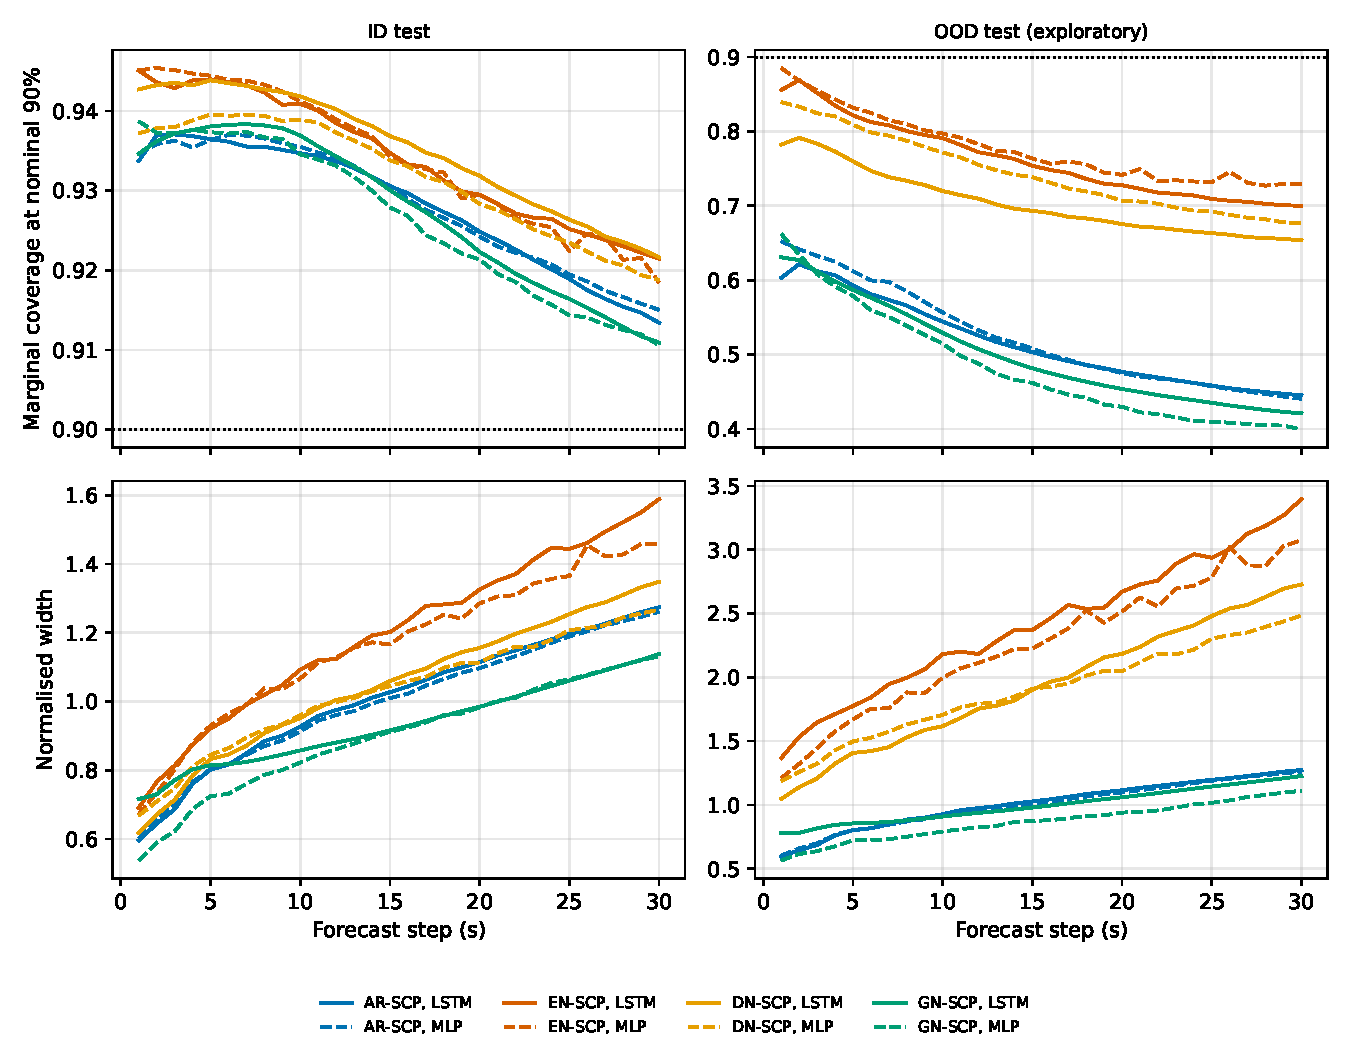
\includegraphics[width=0.92\linewidth]{generated/fig_horizon.pdf}
\caption{Marginal coverage at nominal 90\% (top) and normalised interval width (bottom) by forecast step for the split-conformal constructions; means over three training repeats (no uncertainty bands shown). Left: ID test; right: OOD test (exploratory).}
\label{fig:horizon}
\end{figure}

\subsection{Separating backbone, score and calibration effects}
\label{sec:results-effects}

% generated by src.analysis.report_pub from frozen v3 outputs; do not edit by hand
\begin{table*}[tbp]
\centering
\footnotesize
\caption{Predeclared paired differences (A $-$ B) at nominal 90\%, computed on identical recordings and windows with shared bootstrap draws (2000 cluster resamples of recordings; repeats averaged within each draw). $\Delta$Cov in percentage points; $\Delta$IS = difference in normalised interval score (negative = A better). Values are printed with extra decimals where needed so that no non-zero bound appears as zero. Intervals are descriptive: no multiplicity adjustment, and an interval that includes zero is not evidence of equivalence.}
\label{tab:paired}
\begin{tabular}{lcccc}
\toprule
& \multicolumn{2}{c}{ID test} & \multicolumn{2}{c}{OOD test (exploratory)} \\ \cmidrule(lr){2-3}\cmidrule(lr){4-5}
Pair & $\Delta$Cov (pp) & $\Delta$IS & $\Delta$Cov (pp) & $\Delta$IS \\
\midrule
\multicolumn{5}{l}{\emph{Construction vs.\ AR-SCP on the same backbone (differs in score \emph{and} predictor)}} \\
EN-SCP $-$ AR-SCP, LSTM & 0.6 [-0.5, 2.1] & 0.03 [-0.03, 0.08] & 24.7 [23.6, 25.8] & -1.89 [-2.03, -1.75] \\
EN-SCP $-$ AR-SCP, MLP & 0.6 [-0.4, 1.9] & 0.03 [-0.04, 0.09] & 25.4 [24.4, 26.4] & -2.18 [-2.33, -2.03] \\
DN-SCP $-$ AR-SCP, LSTM & 0.7 [-0.02, 1.6] & -0.06 [-0.12, -0.01] & 18.9 [18.1, 19.6] & -1.77 [-1.88, -1.66] \\
DN-SCP $-$ AR-SCP, MLP & 0.3 [-0.5, 1.4] & -0.09 [-0.17, -0.03] & 22.0 [21.1, 23.1] & -2.09 [-2.22, -1.96] \\
GN-SCP $-$ AR-SCP, LSTM & -0.1 [-1.5, 1.6] & -0.24 [-0.34, -0.17] & -1.6 [-2.9, -0.2] & 0.22 [0.10, 0.33] \\
GN-SCP $-$ AR-SCP, MLP & -0.2 [-1.6, 1.4] & -0.28 [-0.38, -0.20] & -4.1 [-5.5, -2.6] & 0.38 [0.27, 0.49] \\
\multicolumn{5}{l}{\emph{Backbone (MLP $-$ LSTM) within a construction}} \\
AR-SCP & 0.02 [-0.1, 0.2] & -0.01 [-0.02, -0.003] & 0.8 [0.6, 1.0] & -0.06 [-0.09, -0.03] \\
EN-SCP & 0.0005 [-0.1, 0.1] & -0.01 [-0.04, 0.02] & 1.5 [1.3, 1.8] & -0.35 [-0.38, -0.32] \\
DN-SCP & -0.3 [-0.6, -0.04] & -0.05 [-0.07, -0.03] & 4.0 [3.6, 4.4] & -0.38 [-0.42, -0.35] \\
GN-SCP & -0.1 [-0.3, 0.1] & -0.05 [-0.06, -0.04] & -1.7 [-2.1, -1.4] & 0.10 [0.07, 0.14] \\
\multicolumn{5}{l}{\emph{Calibrated $-$ raw band of the same spread}} \\
Ensemble, LSTM & 33.8 [32.7, 34.8] & -0.74 [-0.97, -0.53] & 44.1 [43.6, 44.5] & -4.02 [-4.20, -3.84] \\
Ensemble, MLP & 32.4 [31.1, 33.7] & -0.69 [-0.95, -0.45] & 44.5 [44.0, 45.1] & -4.38 [-4.59, -4.19] \\
Dropout, LSTM & 67.8 [67.3, 68.2] & -1.62 [-1.96, -1.32] & 58.2 [57.7, 58.7] & -6.38 [-6.60, -6.18] \\
Dropout, MLP & 22.1 [21.4, 22.9] & -0.76 [-1.00, -0.55] & 29.5 [29.3, 29.8] & -3.54 [-3.69, -3.41] \\
Gaussian, LSTM & -0.9 [-1.0, -0.8] & -0.01 [-0.02, -0.01] & -1.7 [-1.8, -1.7] & 0.29 [0.28, 0.29] \\
Gaussian, MLP & -0.5 [-0.6, -0.5] & -0.01 [-0.01, -0.004] & -1.1 [-1.1, -1.0] & 0.15 [0.14, 0.15] \\
\bottomrule
\end{tabular}
\end{table*}


The predeclared paired comparisons (Table~\ref{tab:paired}) separate three kinds of difference. First, \emph{calibration}: split conformal changes the coverage of the ensemble and dropout bands by 22--68 percentage points in distribution and 29--58 points under the shift, with lower interval scores. For the Gaussian head, calibration slightly reduces coverage (by 0.5--0.9 points in distribution and 1.1--1.7 points under the shift) and, under the shift, \emph{worsens} the interval score by 0.29 [0.28, 0.29] (LSTM) and 0.15 [0.14, 0.15] (MLP); in distribution its interval score decreases by at most 0.012. The uncalibrated Gaussian bands already exceed the nominal level in distribution. Second, \emph{backbone}: within a construction, the MLP differs from the LSTM by $-1.7$ to $+4.0$ OOD coverage points and by at most 0.05 in ID interval score. Third, \emph{construction}: EN- and DN-SCP exceed AR-SCP on the same backbone by 19--25 OOD coverage points with lower interval scores; GN-SCP covers 1.6--4.1 points less than AR-SCP under the shift, with higher interval scores (by 0.22 and 0.38), although it has lower interval scores than AR-SCP in distribution.

The predeclared construction contrasts compare a spread-normalised score on an ensemble or dropout mean with an absolute-residual score on a single model, so they change both the score and the point forecaster. The stored evaluations also contain absolute-residual conformal intervals on the ensemble, dropout and Gaussian means, which allows a \emph{post hoc} matched comparison (Table~\ref{tab:matched}). With the ensemble mean held fixed, replacing the absolute-residual score by the ensemble-normalised score raises OOD coverage from 50.6\% to 76.2\% (LSTM) and from 51.6\% to 77.7\% (MLP) and lowers the interval score; with the absolute-residual score held fixed, the ensemble mean covers 0.9 (LSTM) and 0.7 (MLP) points less than the single model. For MC dropout, the normalised score on the dropout mean covers 70.4\% and 74.3\% against 50.9\% and 50.8\% for the absolute-residual score on the same mean; the absolute-residual intervals on the dropout mean cover 0.6 (LSTM) and 1.5 (MLP) points less than those of the single deterministic models, which are separately trained networks, so this last contrast is not a pure change of predictor. Because these comparisons were not predeclared and have no recording-level intervals, we treat them as descriptive: in these comparisons, the coverage gain of the spread-normalised scores persisted when the point predictor was held fixed.

% generated by src.analysis.report_pub from frozen v3 outputs; do not edit by hand
\begin{table*}[tbp]
\centering
\footnotesize
\caption{\textbf{Post hoc} (not predeclared) matched comparison at nominal 90\%, from stored evaluation metrics: the same point predictor with two conformal scores, and the same absolute-residual score with two predictors. Values are means over three training repeats; the OOD coverage range over repeats is shown in parentheses (percent). Recording-level intervals were not computed for these contrasts.}
\label{tab:matched}
\begin{tabular}{llccccc}
\toprule
\multicolumn{2}{l}{Predictor / score} & ID cov.\ (\%) & ID IS & OOD cov.\ (\%) (range) & OOD width & OOD IS \\
\midrule
\multicolumn{7}{l}{\emph{LSTM backbone}} \\
Ensemble (5 members) & normalised score & 93.4 & 1.63 & 76.2 (75.2--77.7) & 2.42 & 5.57 \\
Ensemble (5 members) & absolute-residual score & 93.0 & 1.55 & 50.6 (50.5--50.8) & 0.97 & 7.50 \\
MC dropout (200 passes) & normalised score & 93.5 & 1.54 & 70.4 (69.2--71.1) & 1.93 & 5.69 \\
MC dropout (200 passes) & absolute-residual score & 92.8 & 1.60 & 50.9 (50.6--51.4) & 1.01 & 7.61 \\
Gaussian head & normalised score & 92.7 & 1.35 & 49.9 (49.0--51.2) & 1.00 & 7.68 \\
Gaussian head & absolute-residual score & 93.0 & 1.67 & 50.8 (50.3--51.2) & 1.03 & 7.78 \\
Single model (member 0) & absolute-residual score & 92.8 & 1.59 & 51.5 (51.2--51.7) & 1.01 & 7.46 \\
\multicolumn{7}{l}{\emph{MLP backbone}} \\
Ensemble (5 members) & normalised score & 93.4 & 1.61 & 77.7 (77.2--78.7) & 2.26 & 5.22 \\
Ensemble (5 members) & absolute-residual score & 93.1 & 1.54 & 51.6 (51.5--51.7) & 0.97 & 7.40 \\
MC dropout (200 passes) & normalised score & 93.2 & 1.49 & 74.3 (73.8--75.0) & 1.90 & 5.31 \\
MC dropout (200 passes) & absolute-residual score & 92.5 & 1.59 & 50.8 (50.5--51.0) & 1.00 & 7.56 \\
Gaussian head & normalised score & 92.6 & 1.30 & 48.2 (44.6--50.7) & 0.87 & 7.78 \\
Gaussian head & absolute-residual score & 93.0 & 1.56 & 51.7 (51.5--52.1) & 0.97 & 7.46 \\
Single model (member 0) & absolute-residual score & 92.8 & 1.58 & 52.3 (52.1--52.4) & 1.00 & 7.40 \\
\bottomrule
\end{tabular}
\end{table*}


\subsection{Illustrative example}

Fig.~\ref{fig:example} shows one ID test window selected by a rule fixed before evaluation: for the single LSTM of repeat 0 (member 0 of the first LSTM ensemble repeat), we compute for every ID window the per-channel RMSE over the 30 steps divided by the channel's training-target standard deviation, average it over channels, and choose the window whose value is closest to the median over all 106{,}260 windows (ties: lowest window index). The selected window is from recording 20190805-112459, starting at row 2030. It is shown with the four split-conformal constructions on the LSTM backbone. It illustrates the shapes of the intervals and is not evidence of calibration.

\begin{figure}[tbp]
\centering
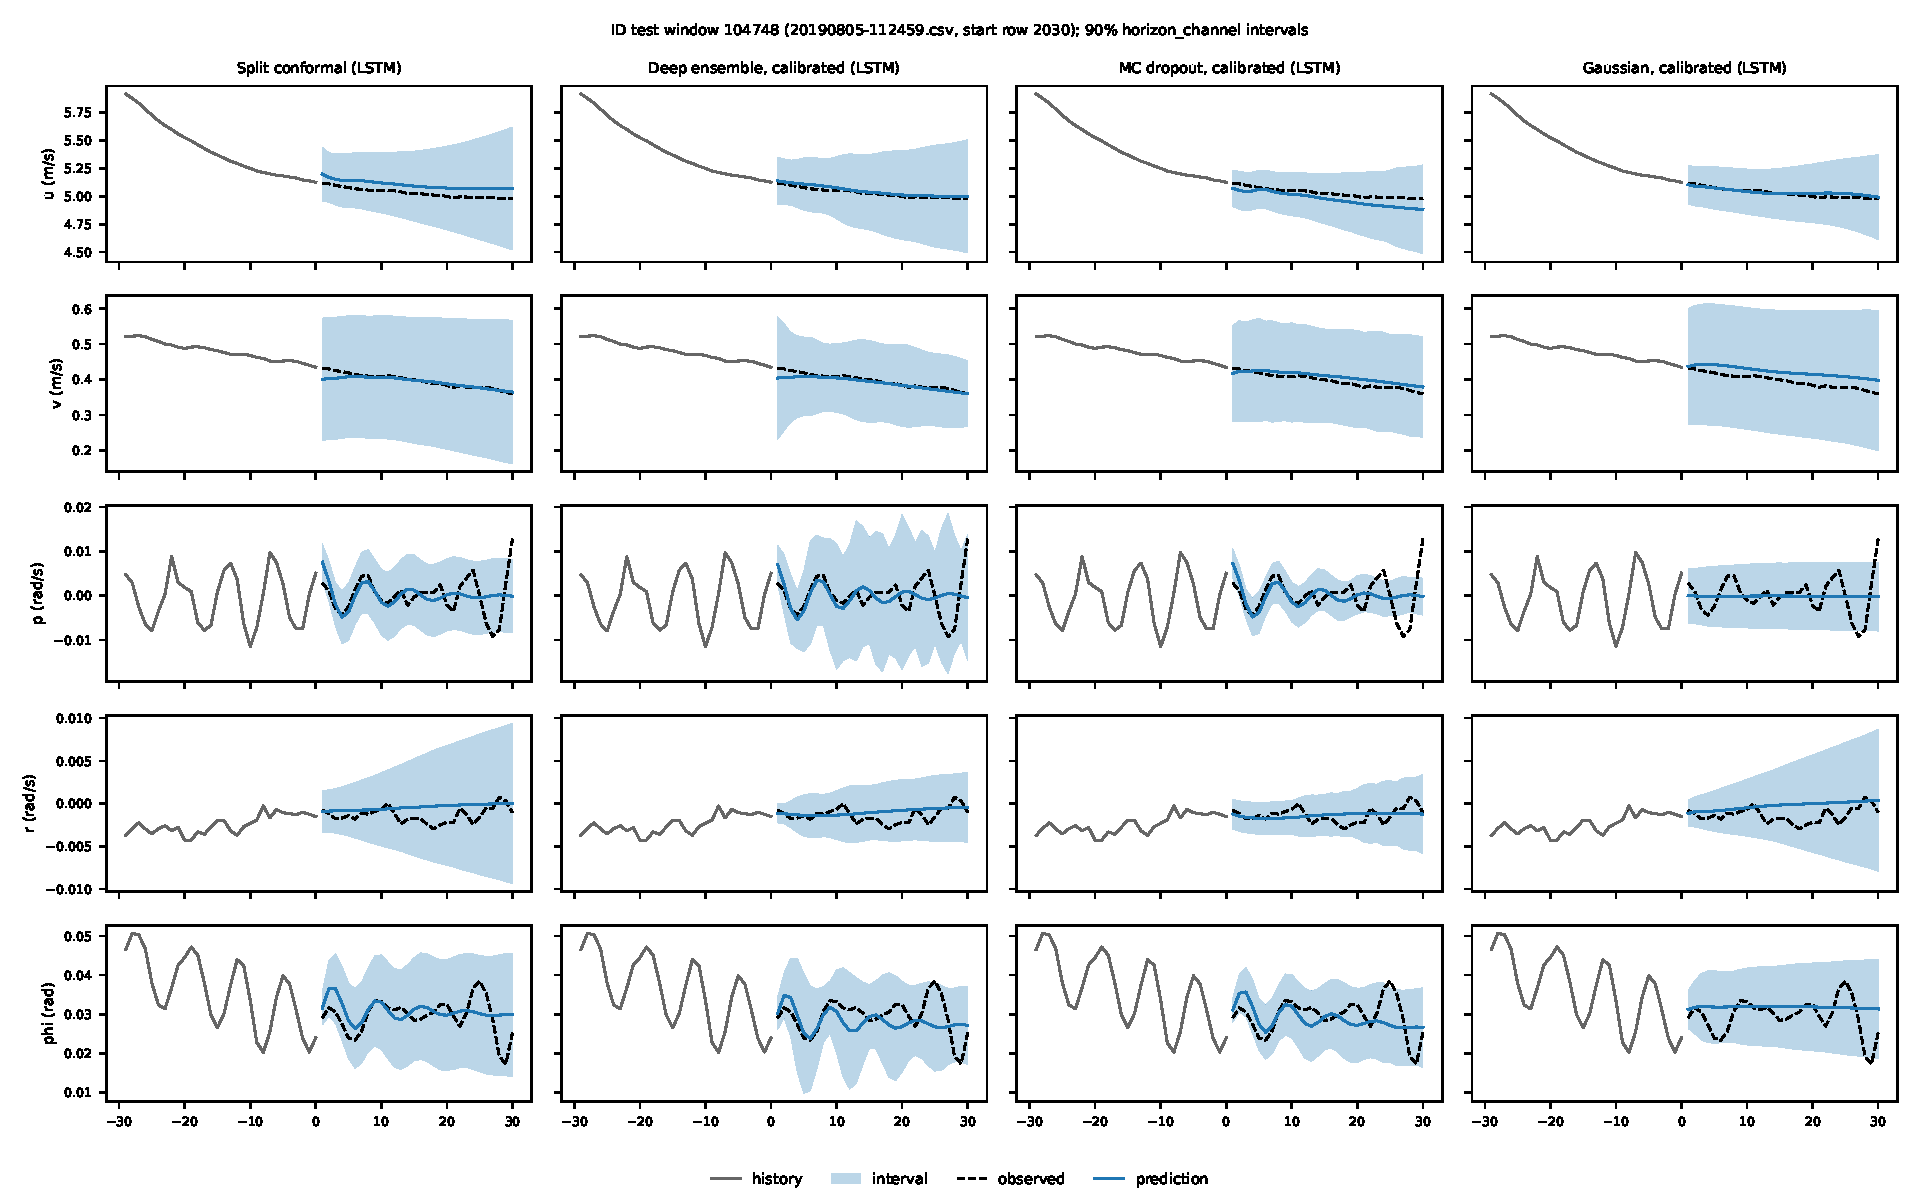
\includegraphics[width=\linewidth]{generated/fig_example_window.pdf}
\caption{Fixed-rule example window from the ID test set (closest to the median channel-averaged normalised RMSE of the reference single LSTM): 30-s history, observed future (dashed), prediction and 90\% split-conformal interval with step- and channel-specific thresholds, for AR-SCP (single LSTM) and EN-, DN- and GN-SCP (LSTM backbone). One realisation of one repeat; not evidence of calibration.}
\label{fig:example}
\end{figure}

% generated by src.analysis.report_pub from frozen v3 outputs; do not edit by hand
\begin{table*}[tbp]
\centering
\footnotesize
\caption{\textbf{Post hoc descriptive} breakdown of ID-test coverage (\%) by nominal level, at the first and last forecast step (nominal 90\%), and simultaneous whole-trajectory coverage (fraction of windows with all 30 steps and 5 channels inside the interval; no construction targets this quantity). Means over three training repeats. At 90\%, the largest range of coverage across repeats is 0.4 percentage points among the split-conformal rows (Ensemble-normalised conformal, MLP) and 1.2 points among the uncalibrated Gaussian rows (Gaussian raw (no calibration), LSTM); these are seed ranges, not recording-level intervals.}
\label{tab:o1}
\begin{tabular}{lccccccc}
\toprule
Construction & 50\% & 80\% & 90\% & 95\% & Step 1 & Step 30 & Trajectory \\
\midrule
Abs-residual conformal, LSTM & 61.4 & 85.6 & 92.8 & 96.3 & 93.4 & 91.3 & 0.40 \\
Abs-residual conformal, MLP & 61.6 & 85.7 & 92.8 & 96.4 & 93.5 & 91.5 & 0.38 \\
Ensemble-normalised conformal, LSTM & 64.1 & 86.7 & 93.4 & 96.7 & 94.5 & 92.1 & 0.23 \\
Ensemble-normalised conformal, MLP & 64.6 & 86.8 & 93.4 & 96.7 & 94.5 & 91.8 & 0.23 \\
Dropout-normalised conformal, LSTM & 62.5 & 86.7 & 93.5 & 96.7 & 94.3 & 92.2 & 0.36 \\
Dropout-normalised conformal, MLP & 62.7 & 86.3 & 93.2 & 96.6 & 93.7 & 91.9 & 0.31 \\
Sigma-normalised conformal, LSTM & 62.5 & 85.7 & 92.7 & 96.3 & 93.5 & 91.1 & 0.18 \\
Sigma-normalised conformal, MLP & 62.7 & 85.6 & 92.6 & 96.2 & 93.9 & 91.1 & 0.16 \\
Gaussian raw (no calibration), LSTM & 69.8 & 88.9 & 93.7 & 96.0 & 94.7 & 91.6 & 0.22 \\
Gaussian raw (no calibration), MLP & 69.5 & 88.4 & 93.2 & 95.5 & 94.2 & 91.7 & 0.18 \\
\bottomrule
\end{tabular}
\end{table*}


\FloatBarrier
% ============================================================
\section{Discussion}
\label{sec:discussion}

\subsection{Main findings and relation to prior work}

Three findings are supported by the benchmark. First, in distribution, the calibrated constructions differ little in coverage, and a closed-form linear model has observed errors similar to those of the neural forecasters; the 30 test recordings do not resolve a difference between them, and no equivalence test was performed. Second, uncalibrated ensemble and MC-dropout spreads are far too narrow to serve as prediction intervals, consistent with the view that such spreads represent disagreement between models rather than the full predictive uncertainty \citep{lakshminarayanan2017, gal2016dropout}; split-conformal calibration on separate calibration recordings removes this under-coverage in distribution. Third, under the operating-condition shift every construction under-covers, as expected from studies of uncertainty under dataset shift \citep{ovadia2019can}, but the size of the shortfall depends on the conformal score: scores normalised by ensemble or dropout spread retain 70--78\% coverage at a nominal 90\%, against about 52\% for the absolute-residual score and 48--50\% for the Gaussian-normalised score.

The difference between the spread-normalised constructions follows from how the spreads respond to the shift. The normalised width of EN-SCP roughly doubles from the ID to the OOD test set (1.20 to 2.42 for the LSTM) and that of DN-SCP rises from 1.05 to 1.93, whereas the GN-SCP width barely changes (0.93 to 1.00) and the AR-SCP width is fixed by construction. In other words, in these data the ensemble and dropout spreads increase on OOD inputs while the learned Gaussian standard deviation does not; this is an observation about the widths, not an identified mechanism. The wider intervals are not merely more conservative: their interval scores, which penalise both width and misses, are also lower under the shift. In distribution, EN-SCP intervals are wider than AR-SCP intervals (normalised width 1.20 vs.\ 1.01 for the LSTM) without a resolved difference in interval score (paired difference 0.03 [$-0.03$, 0.08]), and GN-SCP has the narrowest intervals and lowest interval scores.

Relative to the marine literature, \citet{kim2025mcdropoutroll} evaluated MC-dropout intervals for roll motion; our results add a common calibration set, several constructions and an explicitly characterised, though previously consulted, operating-condition shift for multi-step, multivariate forecasts, but they concern a single simulated vessel and do not transfer directly to measured voyage data.

\subsection{Accuracy and model complexity}

The benchmark provides no evidence that the neural forecasters are more accurate than ridge regression on this task: their observed channel-averaged normalised errors are similar, ridge has the lowest ID surge error, and all learned models degrade by a similar factor under the shift. The inputs contain wind and control signals but no wave elevation or wave force; this omitted forcing may limit what can be predicted from the available history, but the benchmark does not identify how much of the remaining error is irreducible and how much reflects model limitations. The neural models reached their best validation loss within a few epochs; the cause of this early optimum was not investigated. For uncertainty quantification the choice of spread matters more than the choice between the two tested backbones, but the MLP and LSTM are only two architectures that differ in several respects, and no statement is made about architectures in general.

\subsection{Practical implications}

Within the limits of this benchmark: (i) uncalibrated ensemble and dropout spreads should not be used as prediction intervals; (ii) split-conformal calibration on separate calibration recordings yielded conservative marginal coverage in distribution in this dataset, with substantial over-coverage in sway (98.5--99\% at a nominal 90\%) and smaller over-coverage in surge; and (iii) nominal coverage cannot be relied on under a change in operating conditions---the highest coverage observed under the (exploratory) shift studied here was about 78\% at a nominal 90\%. The constructions also differ in cost. A deep ensemble requires training five models; MC dropout requires 200 forward passes per forecast (in a timing pilot on an L40 GPU, 23~s for 31{,}878 windows against 1.2~s for one pass of a single LSTM); the Gaussian head and the absolute-residual construction require a single pass. These observations do not establish suitability for safety-critical use.

\subsection{Limitations}
\label{sec:limitations}

\begin{itemize}
\item \emph{Exploratory OOD evaluation.} The 29 OOD recordings were used in an earlier version of this study to choose which backbones to carry forward. Re-running the benchmark with a frozen protocol does not remove that dependence, and no untouched recordings from the shifted condition exist. All OOD comparisons are therefore exploratory.
\item \emph{Nature of the shift.} The OOD condition differs in speed and propeller shaft speed, extrapolating beyond the training range; sea-state parameters are not available, so effects of speed and sea state cannot be separated.
\item \emph{Exchangeability and coverage.} Windows overlap and calibration comprises nine recordings, so the finite-sample conformal guarantee is not established for these data. In-distribution over-coverage is concentrated in surge and sway and is not explained; the calibration recordings are somewhat slower than the others, which is a hypothesis we did not test.
\item \emph{Marginal intervals.} All intervals target marginal coverage; whole-trajectory coverage is 0.16--0.40. Applications needing simultaneous coverage require other constructions (e.g.\ Bonferroni-type multi-horizon corrections; \citealp{stankeviciute2021conformal}).
\item \emph{Scope.} One simulated vessel; two backbones for the uncertainty comparison; fixed architectures and hyperparameters without tuning; three training repeats; recording-level intervals that do not include between-seed variation; no multiplicity adjustment; the matched score-vs-predictor comparison is post hoc and has no recording-level intervals.
\item \emph{Optimisation.} Checkpoints were selected on validation loss with early stopping; this does not demonstrate convergence of optimisation, and the cause of the early validation optimum was not investigated.
\item \emph{Earlier version.} An unpublished earlier version of this study used a different data pipeline and evaluation protocol; several of its conclusions are not supported by the present benchmark. The differences are documented in the code repository's revision record; because they changed together, their individual effects are not identified.
\item \emph{Units.} The dataset documentation lists the propeller shaft speed in 1/s, but the recorded magnitudes suggest a different convention; this does not affect the models, which use standardised inputs.
\end{itemize}

% ============================================================
\section{Conclusions}
\label{sec:conclusions}

We benchmarked point forecasters and uncertainty constructions for 30-s multi-step forecasts of five motion states of a simulated patrol vessel, in distribution and under an exploratory change in operating conditions, with calibration recordings excluded from fitting, three training repeats and recording-level intervals. In distribution, closed-form ridge regression and the neural forecasters had similar observed errors; uncalibrated ensemble and dropout spreads under-covered severely; and every split-conformal construction covered about 93\% of observations at a nominal 90\%. Under the shift, all learned models lost accuracy by a similar factor, and all constructions under-covered. Conformal scores normalised by ensemble or dropout spread retained the most coverage (70--78\%) with wider intervals but lower interval scores than absolute-residual (50--53\%) or Gaussian-normalised (48--50\%) scores; in post hoc, descriptive matched comparisons this gain persisted when the point predictor was held fixed, and differences between the MLP and LSTM backbones were small. These OOD findings are exploratory. Adaptive or shift-aware conformal procedures \citep{gibbs2021adaptive, tibshirani2019conformal}, simultaneous trajectory intervals, confirmation on untouched operating conditions and measured full-scale data are the most direct next steps.

\FloatBarrier
% ============================================================
\section*{Data and code availability}
The dataset is available from DaRUS \citep{baier2022darus} (doi:10.18419/darus-2905). The code repository (\url{https://github.com/mertoo/phd-p1-darus-uncertainty}) contains the code, configurations, recording-level split manifests, the calibration-selection record, run seeds, the Python environment specification, per-evaluation metrics, bootstrap outputs, and the scripts and commands that regenerate every table and figure of this paper from those outputs. The feature ablation ran at version \texttt{dde1848}, training, evaluation and analysis at \texttt{83585da}; results are archived in \texttt{630baad}, and the manuscript tables and figures are generated at a later version listed in the repository's revision record. Model checkpoints and full prediction arrays (about 16~GB) are not publicly archived; they are available from the corresponding author on request.

\bibliographystyle{cas-model2-names}
\bibliography{bibliography}

\end{document}
